\documentclass[a4paper,12pt]{report}
\usepackage{graphicx}
\usepackage{listings}
\usepackage{amsmath}
\usepackage{color}
\usepackage{titlesec}
\titleformat{\chapter}{}{}{0em}{\bf\LARGE}

\begin{document}
\title{Report}
\author{Martin Moran}
\maketitle

\chapter{Introduction}
[In this section we will introduce the concept of using HPC to study genetics. We must include the motivation of doing this work and place special importance on how HPC can be used to improve this [i.e allow us to achieve this in a reasonable timescale]]

The computational analysis of large genetic datasets is a great challenge to biomedical research. By reading DNA sequences we can study the adaptation of populations to their environment and the occurrence of genetic diseases. However, projects such as the 1000 genomes \cite{1000} and Genome 10K \cite{10K} projects are currently generating data faster than it can be analysed. One of the major priorities of modern biomedical research is overcoming this computational bottleneck to enable key biological problems to be addressed. Methods have been produced, such as the extended haplotype homozygosity \cite{EHH} and integrated haplotype score \cite{iHS}, to investigate these large genetic datasets. 

About 51 million SNPs have been observed in the human population. With the increase in the number of SNPs, the complexity of the problem of calculating iHS is increased. Testing all these individually is time consuming, testing pairs is even more so. In testing pairs the number of combinations grows exponentially as the number of SNPs is increased. For example, if we consider chromosome 22 to have 489,301 SNPs, the number of combinations of pairs would be almost 120 billion. For biological reasons we restrict the analysis to those within 500,000 bases. In this case the numbers of pairs we would analyse would be much less than 120 billion but would still offer a huge challenge for HPC.

The increased in performance in HPC allows us to study larger areas than previously possible. Previously analysis was only feasible in small regions where we have a hypothesis about a gene. The increased power would allow for full chromosomes to be analysed. This would be hypothesis free analysis.

This project is an extension of the program Hapbin which was created by Colin MacLean as part of the MSc for HPC Dissertation in 2014.\cite{hapbin}. It has the functionality to calculate the EHH and iHS for a single locus or a pair of loci. It is written in C++11 with the MPI wrapper MPIRPC.

The aim of this project is to explore efficient means to study combinations of two or more alleles by extending and improving the existing code. A pair of alleles may be positively or negatively selected in combination while the individual alleles are not on their own. Consider the case shown in figure 3.1. Regulatory single nucleotide variant (rSNV) is the change of a single nucleotide bases in a locus which affects the expression of a protein, that is how much of that protein is produced. Coding single nucleotide variants (cSNV) is the change in a location which affects the protein produced. We expect to see negative selection in the case where a rSNV increases the expression of a protein and a cSNV produces a negatively modified version of that protein. 


\chapter{Background}
[We must introduce the genetic concepts used in this dissertation, such as DNA and SNPs. We must also explain EHH, IHH and IHS as well as the concepts of N-wise and conditional analysis.]

\section{Basic Genetics}
Deoxyribonucleic acid (DNA) is a molecule which encodes the genetic instructions used in the development and function of living organisms. DNA is composed of simpler units known as nucleotides. These contain one of four nucleobases: guanine (G), adenine (A), thymine (T) and cytosine (C).

Through the process of transcription and translation, a sequence of three nucleotides are used to encode a single amino acid. These amino acids are built up, using the code of the DNA sequence, into proteins. These proteins perform a large number of functions within living organisms.

DNA is packaged into structures known as chromosomes. Human cells have 23 pairs of chromosomes, 22 pairs of autosomes and one pair of sex chromosomes. Each pair of autosomes contain the same genes, though they may contain different alleles, alternative forms of the same gene. In sexual reproduction half of each pair from two individuals are copied, in a process known as meiosis, and combined to form the chromosomes of the offspring.

\begin{figure}[h!]
  \centering
    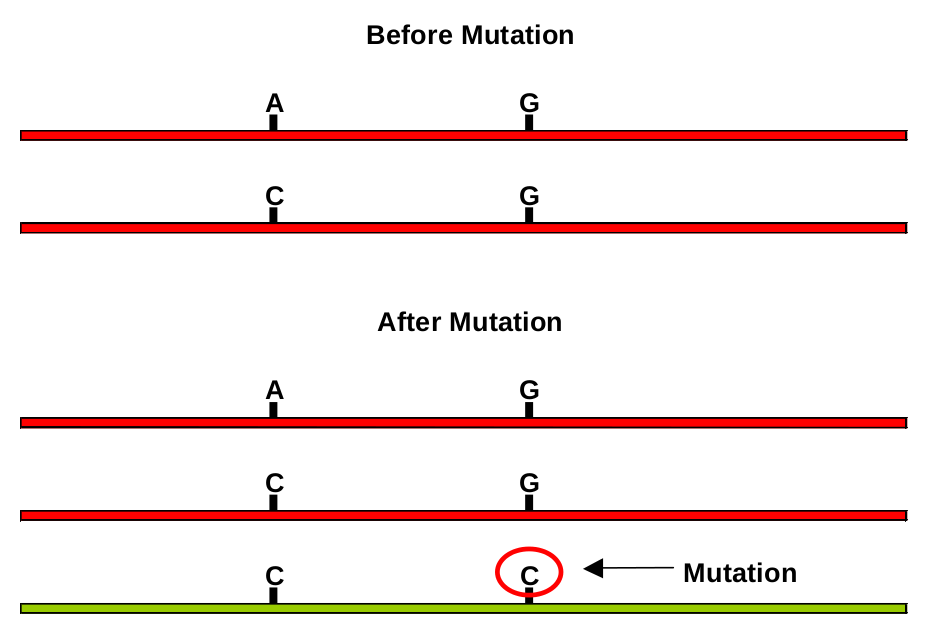
\includegraphics[scale=0.2]{SNP}
  \caption{Mutation which produces SNP}
\end{figure}

A single nucleotide polymorphism (SNP) is the change of a single nucleotide base in a DNA sequence, for example C\underline{G} and C\underline{C}. In this case we say that there are two alleles. Almost all common SNPs have only two alleles. This allows us to represent the SNPs on a chromosome as 1s and 0s in a file. We represent the ancestral allele, the allele before the mutation, as 0 and the derived allele as 1.\cite{selscan} Figure 2.1 shows a mutation which produces a SNP, where a G base is mutated into a C base.

\begin{figure}[h!]
  \centering
    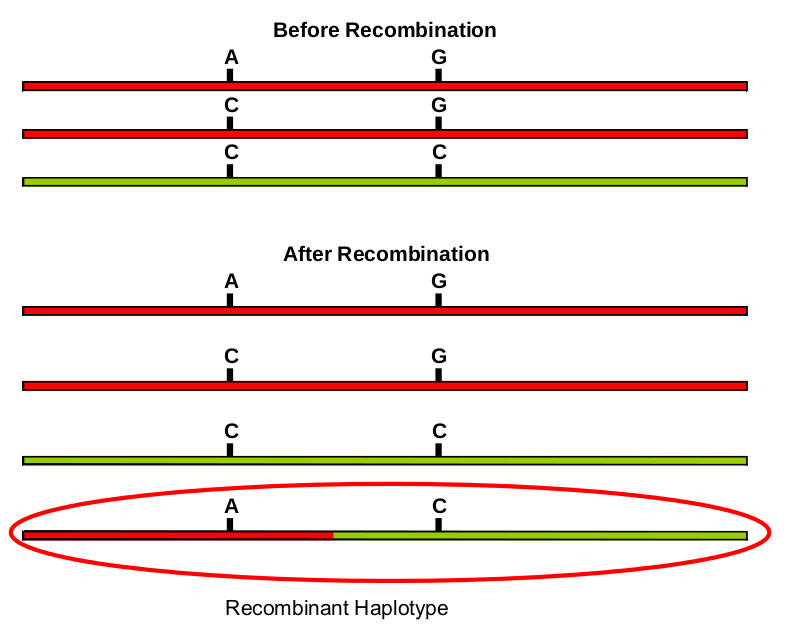
\includegraphics[scale=0.25]{recombination1}
  \caption{Recombination of bases}
\end{figure}


DNA recombination involves the exchange of genetic material either between multiple chromosomes or between different regions of the same chromosome. Figure 2.2 shows an example of recombination. Recombination occurs during meiosis, where genetic information is exchanged between the newly copied chromosomes. This results in offspring inheriting genes from all four grandparents. Recombination produces a new combination of alleles, known as a haplotype.

\section{Extended haplotype homozygosity}

The extended haplotype homozygosity ($EHH$) calculates a measure of the uniqueness of haplotypes at a locus, a position on a chromosome. $EHH$ can be used to study a specific core haplotype, an allele or group of alleles at a locus. If the core haplotype is of length 1 the core haplotype could be either (0) or (1). The equation for $EHH$ with a core haplotype c, extending from the core haplotype $x_0$ to the locus $x_i$, is:
\begin{equation}
EHH_c(x_i) = \sum_{h\in\mathcal{H}_c(x_i)}\dfrac{\binom{n_h}{2}}{\binom{n_c}{2}}
\end{equation}
where $\mathcal{H}_c(x_i)$ is the set of haplotypes with core haplotype c extending to the locus $x_i$, $n_h$ is  the number of observed haplotypes of type $h\in\mathcal{H}_c(x_i)$ and $n_c$ is the number of core haplotypes observed.\cite{EHH}  $\binom{n}{k}$ is known as the binomial coefficient and can be given by the expression $\dfrac{n!}{k!(n-k)!}$.

The EHH algorithm can find regions with low recombination and mutation rates but without comparing these region with other regions we cannot conclude that the region has been positively selected.

\section{Integrated Haplotype Score}

The integrated haplotype homozygosity ($iHH$) is $EHH$ integrated with the trapezoid rule. $iHH$ is given by:
\begin{equation}
\begin{split}
iHH_c = &\sum_{i=1}^{|\mathcal{U}|}\dfrac{1}{2}(EHH_c(x_{i-1})+EHH_c(x_i))g(x_{i-1},x_i)+\\
&\sum_{i=1}^{|\mathcal{D}|}\dfrac{1}{2}(EHH_c(x_{i-1})+EHH_c(x_i))g(x_{i-1},x_i)
\end{split}
\end{equation}
where $\mathcal{U}$ is the set of loci upstream of the core haplotype, $\mathcal{D}$ is the set downstream and $g(x_{i-1},x_i)$ is the genetic distance between the loci $x_{i-1}$ and $x_i$. $EHH_c$ values which are less than 0.05 are truncated.

We need to compare this with the $iHH$ for the haplotypes which do not contain the core haplotype. This would give the unstandardised integrated haplotype score ($uiHS$):
\begin{equation}
uiHS_c = \ln\left(\dfrac{iHH_c}{iHH_{\mathcal{O}_c}}\right)
\end{equation}
$\mathcal{O}_c$ are the haplotypes which do not contain the core haplotype $c$. For core haplotypes of length 1 this would be 1 if the core haplotype is 0 and 0 if the core haplotype is 1.

We must standardise this with haplotypes which have similar core frequencies. The standardised integrated haplotype score ($iHS$) is:
\begin{equation}
iHS_c = \dfrac{uiHS_c-M_p[uiHS_c]}{SD_p[uiHS_c]}
\end{equation}
where $M_p[uiHS_c]$ and $SD_p[uiHS_c]$ are the mean and standard deviation respectively of frequency bin $p$.\cite{iHS}  $p$ is the frequency bin of core haplotype c. If the $iHS$ is higher than expected positive selection is said to have occurred. 
\section{Pairwise and N-wise analysis}
In previous sections we have described EHH and iHS for core haplotypess of length 1. We may instead investigate core haplotypes of length 2 \cite{hapbin}, know as pairwise analysis, or core haplotypes of length N, N-wise analysis.

In pairwise the core haplotype can be one of four haplotypes: (0 0), (0 1), (1 0) or (1 1). The two alleles of the core haplotype do not necessarily need to be beside each other in the haplotype.

\begin{figure}[h!]
\begin{center}
  \begin{tabular}{ | r c c c | c | c c c l |}
    \multicolumn{4}{c}{Downstream} & \multicolumn{5}{c}{Upstream} \\
    \hline
    \ldots & 1 & 0 & 0 & \color{red} 1 & 0 & 1 & 0 & \ldots \\
    \ldots & 0 & 1 & 1 & \color{red} 0 & 0 & 0 & 0 & \ldots \\
    \ldots & 1 & 1 & 0 & \color{red} 1 & 1 & 0 & 1 & \ldots \\
    \hline
  \end{tabular}
    \caption{Upstream and Downstream loci for single locus. Core haplotype in red}
\end{center}
\end{figure}

\begin{figure}[h!]
\begin{center}
  \begin{tabular}{ | r c c c | c c c c | c c c l |}
    \multicolumn{4}{c}{Downstream} & \multicolumn{4}{c}{} & \multicolumn{4}{c}{Upstream} \\
    \hline
    \ldots & 1 & 0 & 0 & \color{red} 1 & 0 & 1 & \color{red} 1 & 0 & 1 & 0 & \ldots \\
    \ldots & 0 & 1 & 1 & \color{red} 0 & 1 & 1 & \color{red} 1 & 0 & 0 & 0 & \ldots \\
    \ldots & 1 & 1 & 0 & \color{red} 1 & 0 & 0 & \color{red} 1 & 1 & 0 & 1 & \ldots \\
    \hline
  \end{tabular}
      \caption{Upstream and Downstream loci for pairwise. Core haplotype in red}
\end{center}
\end{figure}

\begin{figure}[h!]
\begin{center}
  \begin{tabular}{ | r c c c | c c c c | c c c l |}
    \multicolumn{4}{c}{Downstream} & \multicolumn{4}{c}{} & \multicolumn{4}{c}{Upstream} \\
    \hline
    \ldots & 1 & 0 & 0 & \color{red} 1 & \color{red} 0 & 1 & \color{red} 1 & 0 & 1 & 0 & \ldots \\
    \ldots & 0 & 1 & 1 & \color{red} 0 & \color{red} 1 & 1 & \color{red} 1 & 0 & 0 & 0 & \ldots \\
    \ldots & 1 & 1 & 0 & \color{red} 1 & \color{red} 0 & 0 & \color{red} 1 & 1 & 0 & 1 & \ldots \\
    \hline
  \end{tabular}
        \caption{Upstream and Downstream loci for 3-wise. Core haplotype in red}
\end{center}
\end{figure}

When finding the $EHH_c$ of a core haplotype of length two or more, for downstream $EHH$ values we find the $EHH$ from the lowest allele. Likewise for upstream $EHH$ values, we find the $EHH$ from the highest allele. Alleles between the highest and lowest alleles of the core haplotype are ignored in all the calculations. Figure 2.3 shows an example of upstream and downstream loci for a single core locus. Figure 2.4 shows this for pairwise. Figure 2.5 shows this for 3-wise. When standardising the $uiHS$ for pairwise and N-wise we must standardise with haplotypes with the same frequency and same number of ancestral and derived alleles.

\chapter{Design}
[In this section we will discuss the overall design of the program. We must explain the key areas of the original program and discuss how these are changed to implement N-wise and conditional analysis]

\section{EHH}


\section{IHS}

\chapter{Implementation}
[This section will contain the specific tools used to implement the program. We should discuss the use of openMP and MPIRPC specifically.]

\chapter{Results and Analysis}
[This section should present results and benchmarks of the program. We will want to benchmark the program on Archer. These should be analysed with conclusions taken from  these results]

Will need to discuss the datasets used. Will also need to discuss the hardware used.

Section on the effect of of changing from pairwise code to N-wise in terms of memory usage and performance. Main change affecting this would be the change from static to dynamic memory.

Section on the scaling of memory usage and performance as the size of the datasets are increased.

Provide EHH plot for single, pairwise and 3-wise. Will want to discuss which SNPs appear to be positively selected etc.


\chapter{Future Work}
[In this section we will set out some of the possible avenues of study to follow in future work.]

\section{Conditional Analysis}
Finding a pair of SNPs which have a high pairwise IHS does not necessarily mean that they are being positively selected. The location of SNPs can effect their IHS. If a nearby SNP is being positively selected it can cause SNPs physically near that locus to appear to be positively selected for. It is assumed that a single SNP is more likely to be positively selected for than a pair of SNPs. In this case we must conditionally analyse the SNP pairs to see if it is being affected by the the nearby SNPs. 

\begin{figure}[h!]
  \centering
    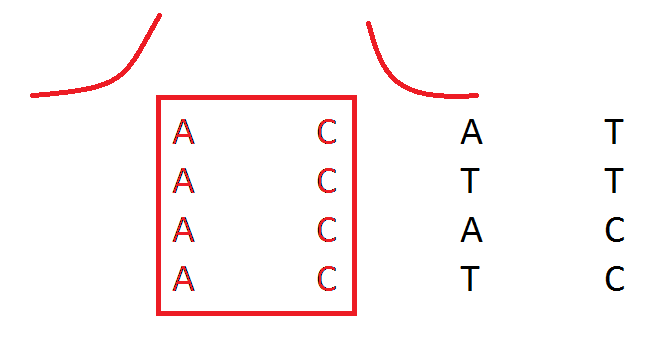
\includegraphics[scale=0.5]{conditional1}
  \caption{Pairwise IHS of first and second SNP}
\end{figure}

We begin by performing the pairwise IHS for a pair of alleles, as shown in figure 1. If we find that this is a high IHS we must investigate nearby single SNPs for their effect on the pair of SNPs. We find the IHS for SNPs within a certain distance of the pairwise IHS as shown in figure 2.

\begin{figure}[h!]
  \centering
    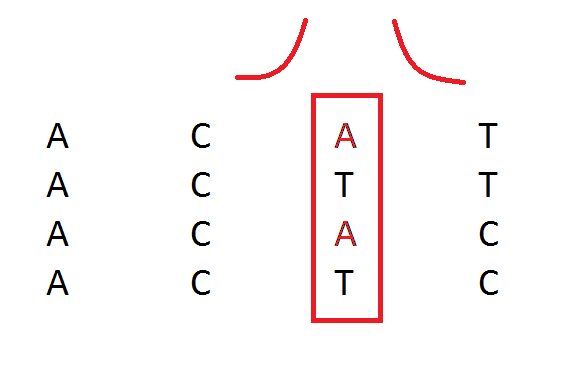
\includegraphics[scale=0.5]{conditional2}
  \caption{IHS of third SNP}
\end{figure}

\newpage
We precondition the pair of SNPs with respect to these single SNPs. This means we find the IHH of the original pair of SNPs who also have the allele of the single SNP which we have found to have high IHS as shown in figure 3. We also find the IHS for the pair without this SNP. If we find that the IHH of the the preconditioned pair with the SNP is similar to the IHH without the SNP we can deduce that the pair of SNPs are being positively selected independently of that SNP. If it is higher we can deduce that the locality of the pair of SNPs to the positively selected SNP is causing the high pairwise IHS.

\begin{figure}[h!]
  \centering
    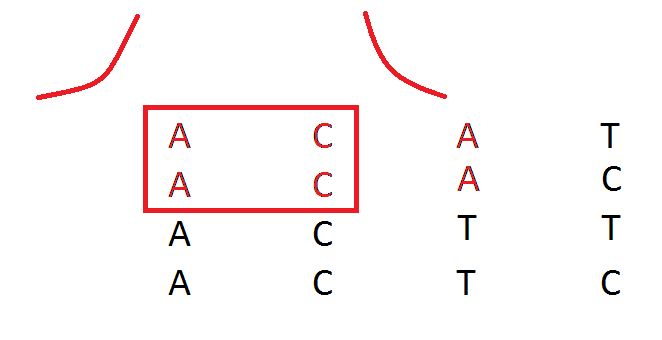
\includegraphics[scale=0.5]{conditional4}
  \caption{Pairwise IHH of first and second SNP preconditioned  with respect to A in the third SNP}
\end{figure}

[I am aware that I need a better way of representing IHS and IHH, as currently it confuses the imagery with EHH]

\chapter{Conclusions}
[In this section we will present some conclusions to the work done for the dissertation]

\begin{thebibliography}{9}

\bibitem{1000}
http://www.1000genomes.org/

\bibitem{10K}
https://genome10k.soe.ucsc.edu/

\bibitem{EHH}
Sabeti, Pardis C., et al. "Detecting recent positive selection in the human genome from haplotype structure." Nature 419.6909 (2002): 832-837.

\bibitem{iHS}
Voight, Benjamin F., et al. "A map of recent positive selection in the human genome." PLoS biology 4.3 (2006): e72.


\bibitem{selscan}
Szpiech, Zachary A., and Ryan D. Hernandez. "selscan: an efficient multi-threaded program to perform EHH-based scans for positive selection." Molecular biology and evolution (2014): msu211.


\bibitem{hapbin}
MacLean, Colin. "Hapbin: An Efficient Method for Calculating the EHH and iHS of Genetic Datasets." HPC Dissertation (2014).


\end{thebibliography}


\end{document}